\section{Technische Grundlagen}
%Elias Zusammenfassung kapitel
In den technischen Grundlagen wird zuerst der physikalische Zusammenhang für das Messprinzip erläutert. Nachfolgend wird gezeigt wie die Signalaufbereitung funktioniert.

\subsection{Hintergrund Messung}%Marc 1 Seite
Die Leistung kann auf verschiedene Arten gemessen werden. Für das Projekt wurde ein indirektes Messverfahren gewählt. Das Gerät misst die Leistung über den Momentanstrom und die Momentanspannung. Dabei wird folgende Formel verwendet.

\begin{equation}
	p(t) = u(t) \cdot i(t)
\end{equation}
\label{eq:Momentanleistung}

Damit kann die Leistung an einem bestimmten Zeitpunkt $t$ berechnet werden. Das Leistungsmessgerät soll jedoch die mittlere Leistung über zehn Sekunden berechnen. Um dies zu erreichen berechnet der Mikrocontroller die mittlere Leistung. Die folgende Grafik zeigt den dafür verwendeten Algorithmus.
\begin{figure}[H]
\begin{center}
	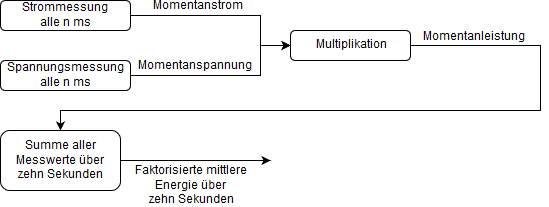
\includegraphics[width=100mm]{images/messung_schematisch.png}
	\caption{Algorithmus um mittlere Leistung zu berechnen} %picture caption
	\label{fig:berechnung_P}
\end{center}
\end{figure}

Wie in Abbildung \ref{fig:berechnung_P} ersichtlich, wird der Momentanstrom und die Momentanspannung alle \textbf{n} Sekunden miteinander multipliziert und die dabei erhaltene Momentanleistung über zehn Sekunden aufsummiert. Dieser Wert enspricht der faktorisierten geflossenen Energie über zehn Sekunden. Begründet ist dies durch folgende mathemetische Umformung.

\begin{equation}
	E = p(t) \cdot \Delta t
\end{equation}
\label{eq:energie1}

Mit der Annäherung, dass die Leistung $p(t)$ im Zeitraum zwischen zwei Messungen $\Delta t$ konstant ist, und unter Berücksichtigung der Formel \ref{eq:Momentanleistung}, ergibt sich folgende Berechnung der Energie.

\begin{equation}
	E_n = u_n \cdot i_n \cdot \Delta t
\end{equation}
\label{eq:energie2}

mit	$u_n, i_n = n $te Messung des Stromes und der Spannung.

Wenn nun alle $E_n$ aufaddiert werden, ergibt sich die Energie über zehn Sekunden. Dabei kann $\Delta t$ ausmultipliziert werden.

\begin{equation}
	E_{10s}\quad = \sum_{n=1}^{ \frac{10s}{\Delta t} } E_n \quad = \quad \sum_{n=1}^{ \frac{10s}{\Delta t} } u_n \cdot i_n \cdot \Delta t \quad = \quad \Delta t \sum_{n=1}^{ \frac{10s}{\Delta t} } u_n \cdot i_n
\end{equation}
\label{eq:energie3}


\begin{equation*}
	\frac{E_{10s}}{\Delta t} = \sum_{n=1}^{ \frac{10s}{\Delta t} } u_n \cdot i_n \quad = \quad aE
\end{equation*}
	
Aus der vom Microkontroller berechneten Wert $aE$ lässt sich unter der Verwendung der Formel $ \overline{P} = \frac{E}{t} $ die mittlere Leistung über zehn Sekunden $\overline{P}$ wie folgt berechnen.

\begin{equation}
	\overline{P}_{10s} = \frac{aE}{\Delta t \cdot 10s}
\end{equation}
\label{eq:mittlere_Leistung}
%%%%%%%%%%%%%%%%%%%%%%%%%%%%%%%%%%%%%%%%%%%%%%%%%%%%%%%%%%%%%%%%%%%%%%%%%%%

\subsection{Signalaufbereitung}\label{subsec:Signalaufbereitung}%Elias 1 Seite
Die Signalaufbereitung passt die Messsignale an die Anforderungen des Analog-Digital-Wandlers, kurz ADC, an. Dieser erwartet ein Signal 0V bis 5V. Jedoch ist der Spannungsabfall über den Mess-Schunts um Faktor 10 bis 160 kleiner. Diese Signalaufbereitungs-Strecke ist für die Strommessung und die Spannungsmessung identisch. Der einzige Unterschied zwischen den verschiedenen Signalen liegt in der Verstärkung.

\begin{figure}[H]
\begin{center}
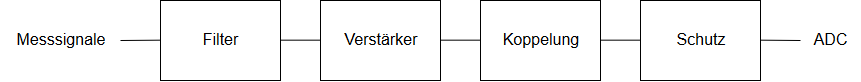
\includegraphics[width=0.9\textwidth]{images/Technische_Grundlagen_Signalaufbereitung.png}
\caption{Signalaufbereitungsstrecke}
\end{center}
\end{figure}

\subsubsection*{Filter}
Die Filter befreien das Messsignal von unerwünschten Signalanteilen. Da im Projektauftrag gefordert wird, dass harmonische Oberwellen ab 5kHz nicht gemessen werden, werden Filter diese Oberwellen entfernen. Dafür wurden Tiefpass-Filter 1. Ordnung verwendet.
\subsubsection*{Verstärkung}
Um die Messsignale auf eine brauchbare Grösse zu bringen, sind nicht-invertierende Verstärker verwendet worden. Diese bringen den Vorteil, dass pro Messstrecke nur ein Operationsverstärker benötigt wird.
\subsubsection*{Koppelung}
Das erwartete Messsignal ist eine sinusartige Schwingung. Dadurch wird das Signal keinen DC-Anteil besitzen. Da der ADC Spannungen von 0 bis 5V fordert, muss das Messsignal angehoben werden.
\subsubsection*{Schutz}
Es ist eine Schutzschaltung eingebaut, um den ADC gegen Über- und Unterspannungen zu schützen. Diese entstehen in der Verstärkerschaltung bei den Messbereichen für kleine Ströme, wenn grosse Ströme gemessen werden.

\pagebreak